\tikzstyle{decision} = [diamond, draw, fill=blue!20,
    text width=6em, text badly centered, inner sep=0pt]
\tikzstyle{block} = [rectangle, draw, fill=blue!20,
    text width=6em, text centered, rounded corners, minimum height=4em]
\tikzstyle{line} = [draw, very thick, color=black!50, -latex']
\tikzstyle{cloud} = [draw, ellipse,fill=red!20, 
    minimum height=2em]
\tikzstyle{noArrow} = [draw, very thick, color=black!50]

\begin{tikzpicture}[scale=2, node distance = 4cm, auto]
	% Nodes
	\node (monitor) {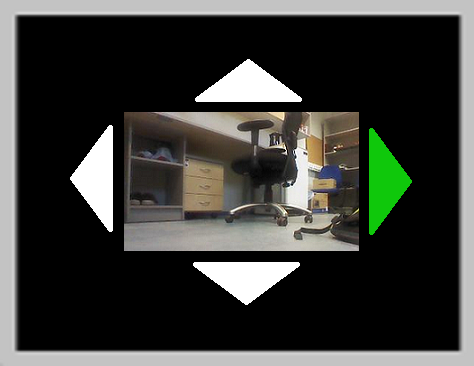
\includegraphics[width=4cm]{arrows_chosen.png}};
	\node [below of=monitor] (brain) {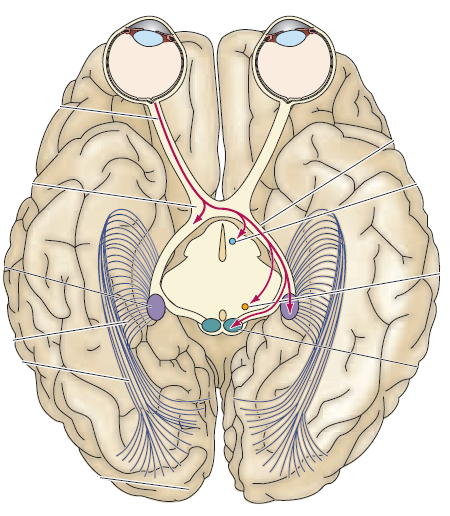
\includegraphics[width=2.5cm]{visual_pathway2.png}};
	%\node [below of=brain, node distance=2cm] {\includegraphics[width=1cm]{electrode.png}};
	\node [block, right of=brain] (emotiv) {Emotiv EPOC headset};
	\node [block, right of=emotiv] (processing) {signal processing};
	\node [block, right of=processing] (extraction) {feature extraction};
	\node [block, above of=extraction] (identification) {target identification};
	\node [left of=identification, node distance=6cm] (robot) {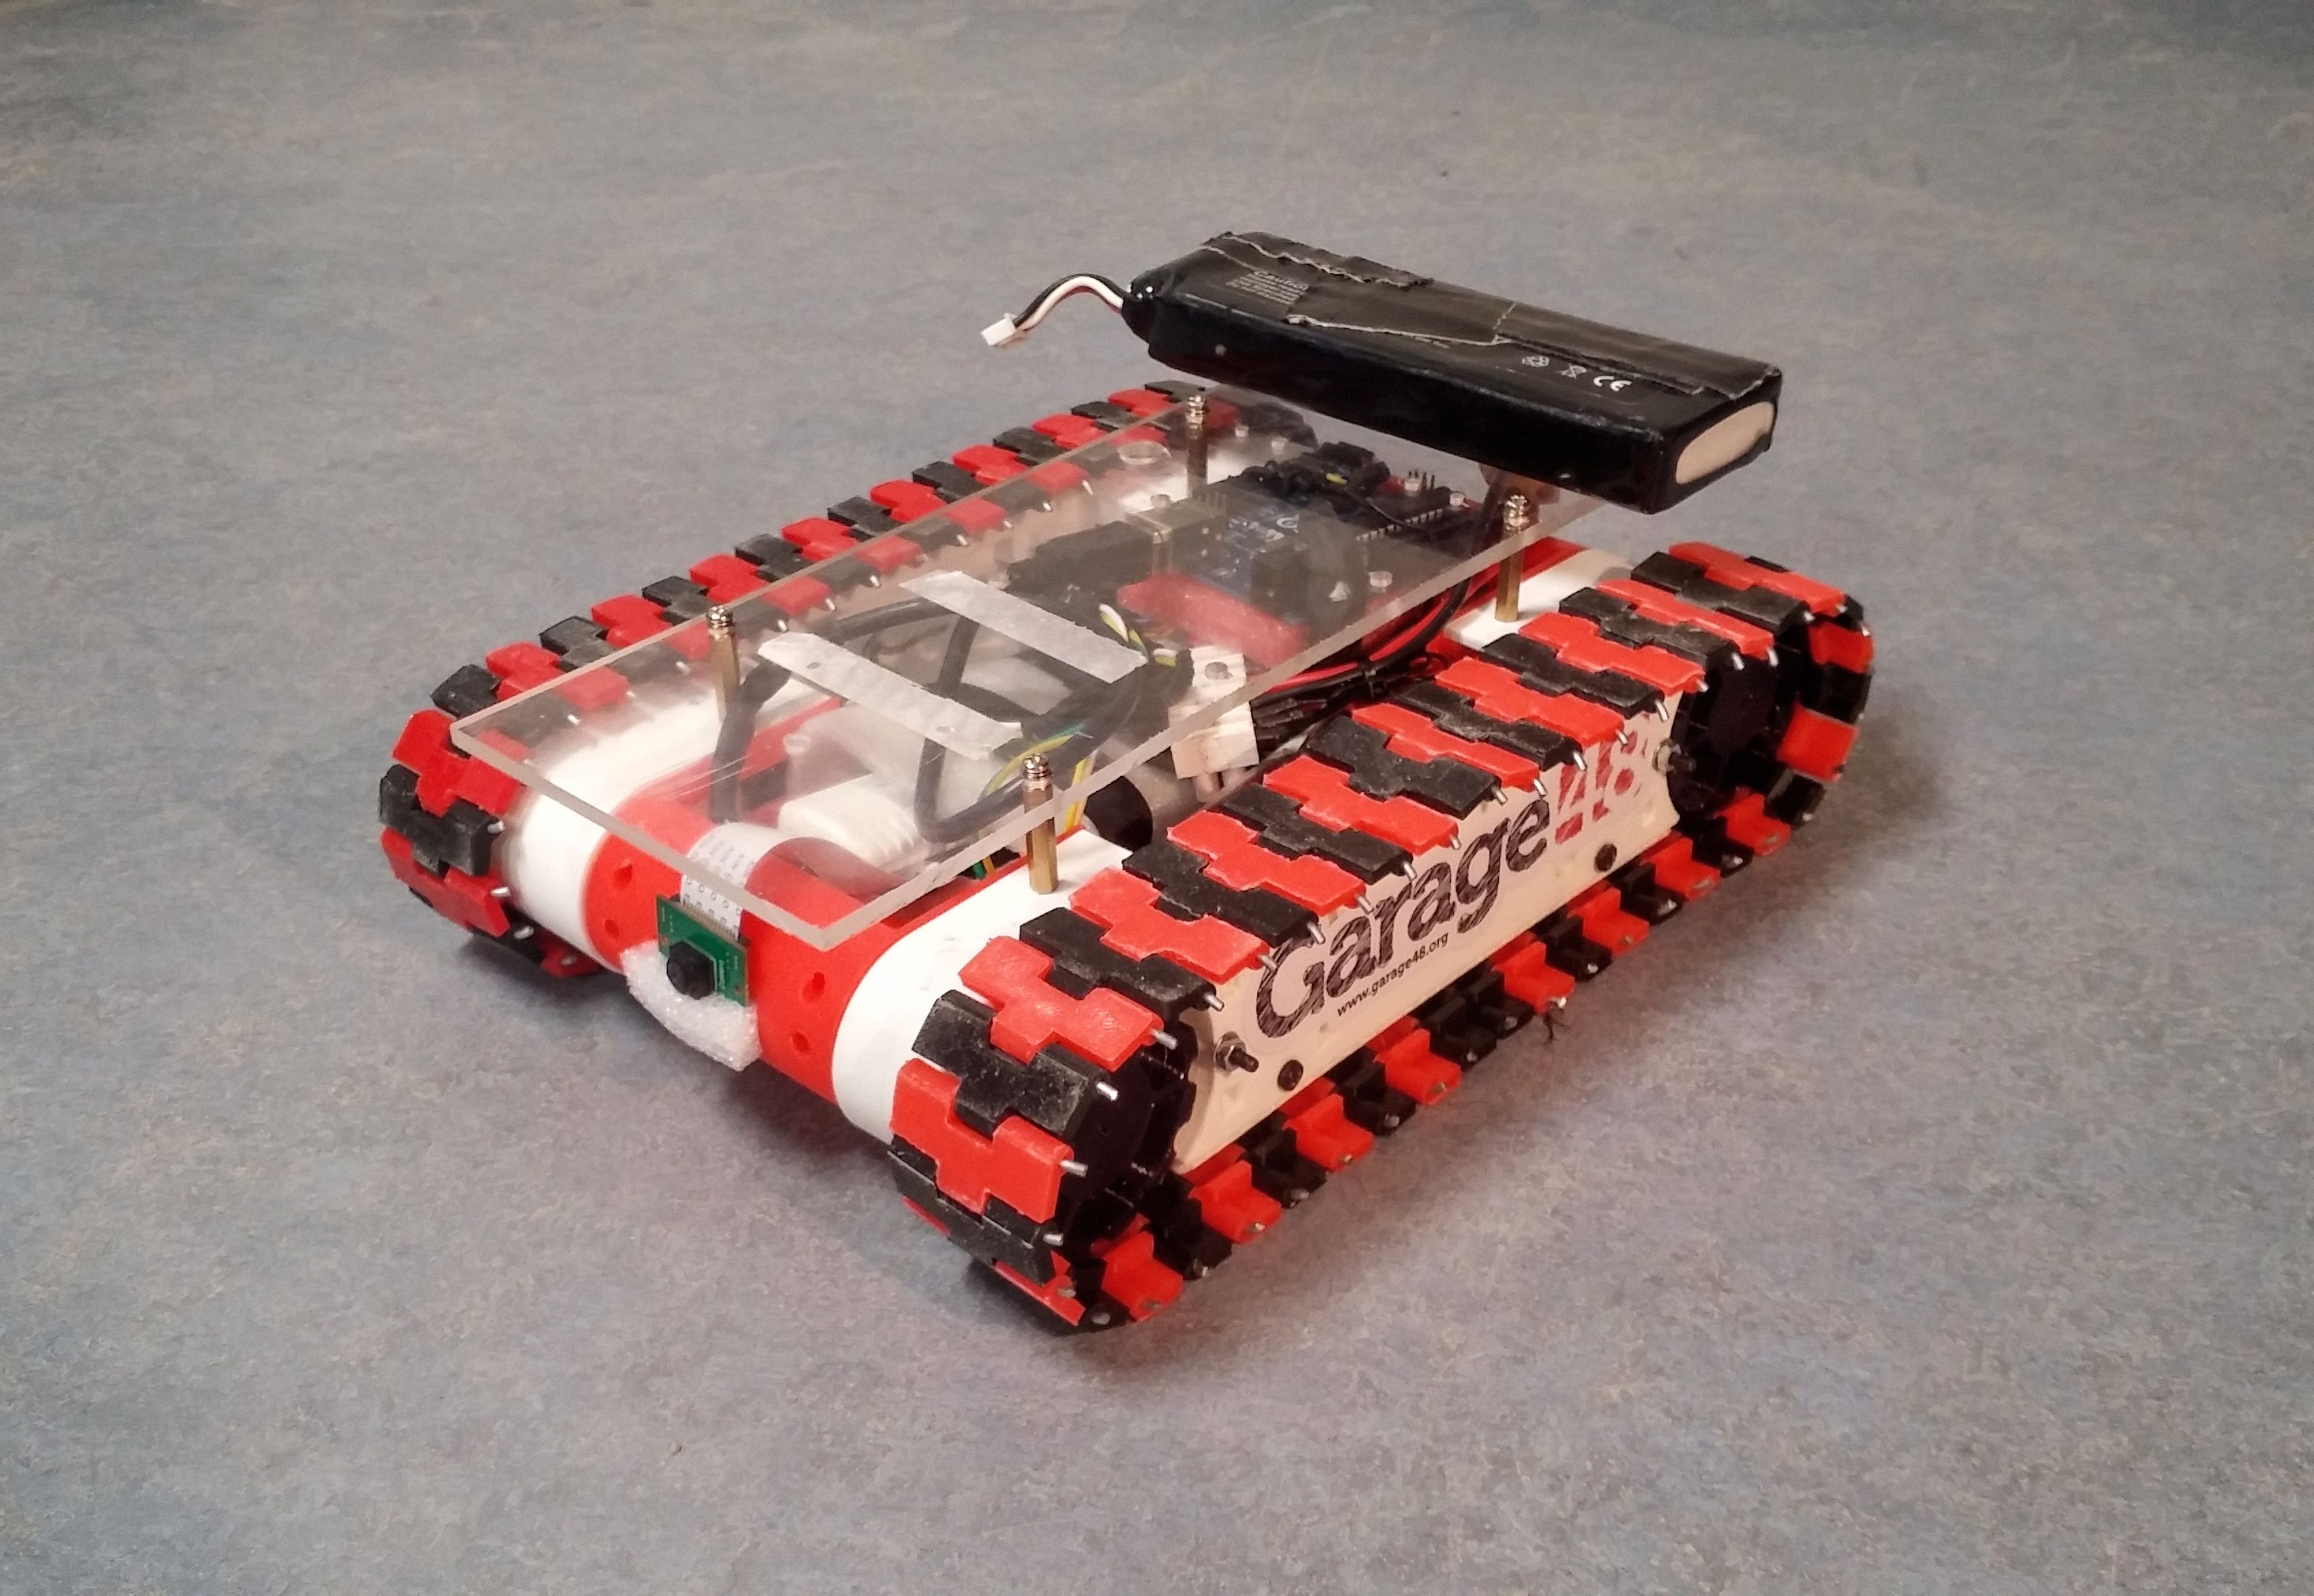
\includegraphics[width=4cm]{robot.jpg}};
	
	\coordinate [above of=robot, node distance=2cm] (dummy);
	\coordinate [left of=dummy] (dummyLeft);
	\coordinate [right of=dummy] (dummyRight);
	
	% Arrows
	\path [noArrow] (identification) -- (dummyRight);
	\path [noArrow] (dummyRight) -- node [color=black, pos=0.5, above] {visual and auditory feedback} (dummyLeft);
	\path [line] (dummyLeft) -- (monitor);
	\path [line] (identification) -- node [color=black, above] {command} (robot);
	\path [line] (extraction) -- (identification);
	\path [line] (processing) -- (extraction);
	\path [line] (emotiv) -- (processing);
	\path [line] (brain) -- (emotiv);
	%\path [line] (threshold) -- node [near start, color=black] {yes} (add);
	%\path [line] (dummyStopRight) -- (new);

\end{tikzpicture}
